\subsection{Intelligence Artificielle et NPC}
Il s'agit de Renaud-Dov qui a réalisé l'implémentation de l'IA.
Pour rendre notre jeu plus vivant et permettre aux joueurs de se méler dans la foule,
il nous fallait créer des IA se déplacant dans la ville.
Pour cela, nous avons décider d'utiliser des NavMesh pour créer des zones où les 
NPC peuvent se balader d'un point A vers un point B.
Pour ne pas rendre leur comportement linéaire et sans saveur,
ils se déplacent de manière aléatoire  vers un point quelconque défini dans une liste de coordonées.
Aucun NPC n'aura donc le même trajet.\\

L’outil de navigation est assez poussé, et permet de définir les dimensions des personnages,
ainsi que la hauteur de laquelle ils peuvent sauter et les pentes qu’ils peuvent emprunter.
Ici, la pente maximale est de 33.4°, mais si ce chiffre avait été plus élevé,
les pentes sur la capture d’écran seraient devenues bleues, et les personnages auraient pu
monter sans utiliser les escaliers (ce qui n’est évidemment pas le but).


Pour rendre ces IA plus humaines, les joueurs peuvent les bousculer et les étourdir en courant vers eux.
Ils reprenent leur trajet au bout de quelques secondes. Il faudra ainsi, dans les prochaines versions, améliorer la navigation afin que le chemin emprunté ne soit pas toujours le plus court. 
\newline

Plusieurs problèmes se posent actuellement avec l'utilisation des NavMesh:
\begin{itemize}
    \item L'IA calcule le chemin le plus court, et n'essaie pas de se déplacer sur le côté si d'autres IA marchent dans le sens contraire.
    Par exemple, si l'ont met deux escaliers cote à côte, toutes les IA vont prendre l'escalier le plus proche et donc se bloquer.\\
    \begin{figure}[hbt!]
        \centering
        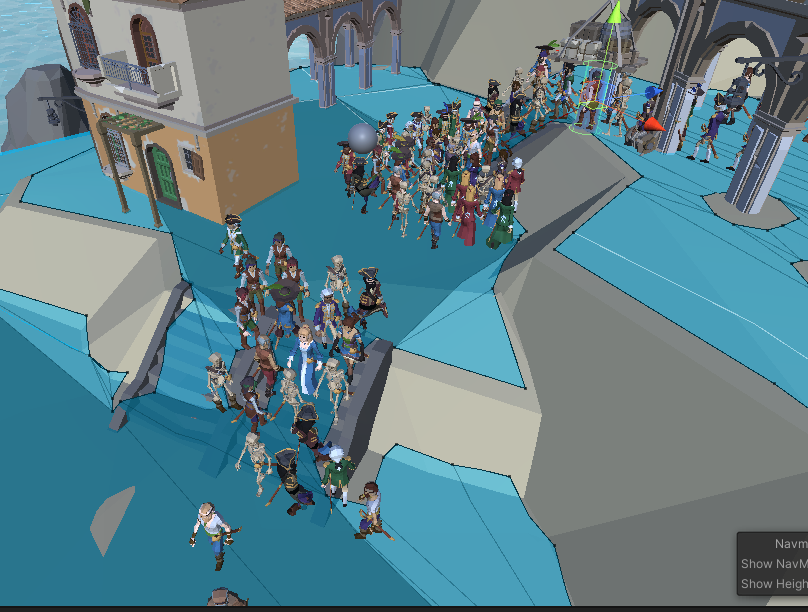
\includegraphics[scale=0.3]{ia_stairs_bug.png}
        \caption{Problème rencontré lorsque de nombreuses IA vont au même endroit}
    \end{figure}
\end{itemize}